\documentclass[12pt,a4paper]{report}
\PassOptionsToPackage{table}{xcolor}

% ============================================================
% TEMPLATE LAPORAN TUGAS BESAR
% Mata Kuliah IoT Cerdas -- S2 Teknik Elektro
% Diadaptasi dari template Buku TA S1 (Deco Aprilianis)
% ============================================================

% -------------------------
% Paket utama
% -------------------------
\usepackage[utf8]{inputenc}
\usepackage[english]{babel}
\usepackage{float}
\usepackage{needspace}
\usepackage{tocloft}
\usepackage{pdfpages}
\usepackage{pdflscape}
\usepackage{longtable}
\usepackage{booktabs}
\usepackage{amsmath}
\usepackage{amssymb}
\usepackage{indentfirst}
\usepackage{tabularx}
\usepackage{array}
\usepackage{cite}
\usepackage{caption}
\usepackage{notoccite}
\usepackage{geometry}
\usepackage{graphicx}
\usepackage{tikz}
\usetikzlibrary{arrows.meta,positioning,shapes.geometric,calc,fit}
\usepackage{times}
\usepackage{setspace}
\usepackage{sectsty}
\usepackage{enumitem}
\usepackage{titlesec}
\usepackage{xurl}
\usepackage{hyperref}
\usepackage{listings}
\usepackage{xcolor}

\hypersetup{hidelinks, colorlinks=false, pdfborder={0 0 0}}
\makeatletter
\newcommand{\printtoccontents}{\@starttoc{toc}}
\makeatother

% -------------------------
% Konfigurasi listings (source code)
% -------------------------
\lstdefinestyle{cstyle}{
    language=C,
    basicstyle=\footnotesize\ttfamily,
    keywordstyle=\bfseries\color{blue!70!black},
    commentstyle=\itshape\color{gray},
    stringstyle=\color{orange!80!black},
    numbers=left,
    numberstyle=\tiny\color{gray},
    stepnumber=1,
    numbersep=8pt,
    frame=single,
    breaklines=true,
    tabsize=2,
    showstringspaces=false,
    captionpos=b
}
\lstdefinestyle{pythonstyle}{
    language=Python,
    basicstyle=\footnotesize\ttfamily,
    keywordstyle=\bfseries\color{blue!70!black},
    commentstyle=\itshape\color{gray},
    stringstyle=\color{orange!80!black},
    numbers=left,
    numberstyle=\tiny\color{gray},
    stepnumber=1,
    numbersep=8pt,
    frame=single,
    breaklines=true,
    tabsize=4,
    showstringspaces=false,
    captionpos=b
}

% -------------------------
% Metadata yang perlu diganti
% -------------------------
\newcommand{\JudulTA}{Sistem Monitoring Suhu Berbasis IoT Cerdas Menggunakan ESP32-S3, Sensor DS18B20, ThingSpeak, dan Random Forest Regressor}
\newcommand{\JudulTAInggris}{Smart IoT-Based Temperature Monitoring System Using ESP32-S3, DS18B20 Sensor, ThingSpeak, and Random Forest Regressor}
\newcommand{\NamaMahasiswa}{Deco Aprilianis}
\newcommand{\NIMMahasiswa}{1102223137}
\newcommand{\ProgramStudi}{S2 Teknik Elektro}
\newcommand{\Kelas}{S2TE-42-RB1}
\newcommand{\Fakultas}{Fakultas Teknik Elektro}
\newcommand{\Universitas}{Universitas Telkom}
\newcommand{\Kota}{Bandung}
\newcommand{\TahunAkademik}{2026}
\newcommand{\MataKuliah}{IoT Cerdas}
\newcommand{\DosenPengampu}{Dr.Eng. Ir. Indra Chandra, S.Si., M.Si.}
\newcommand{\NIPDosen}{[NIP Dosen]}
\newcommand{\TanggalPengumpulan}{22 Juni 2026}

% -------------------------
% Format caption
% -------------------------
\captionsetup[figure]{name=Gambar,labelsep=space,justification=centering,singlelinecheck=false}
\captionsetup[table]{name=Tabel,labelsep=space,justification=centering,singlelinecheck=false}
\AtBeginDocument{%
  \renewcommand{\tablename}{Tabel}%
  \renewcommand{\figurename}{Gambar}%
  \renewcommand{\lstlistingname}{Kode}%
}

% -------------------------
% Format halaman dan spasi
% -------------------------
\geometry{
    top=3cm,
    bottom=3cm,
    left=4cm,
    right=3cm
}
\onehalfspacing
\setlength{\emergencystretch}{2em}
\setlength{\parindent}{1.25cm}

% -------------------------
% Format nomor BAB, section, tabel, gambar, persamaan
% -------------------------
\renewcommand{\thechapter}{\Roman{chapter}}
\renewcommand{\thesection}{\arabic{chapter}.\arabic{section}}
\renewcommand{\thesubsection}{\thesection.\arabic{subsection}}
\renewcommand{\thesubsubsection}{\thesubsection.\arabic{subsubsection}}
\renewcommand{\thetable}{\arabic{chapter}.\arabic{table}}
\renewcommand{\thefigure}{\arabic{chapter}.\arabic{figure}}
\renewcommand{\theequation}{\arabic{chapter}.\arabic{equation}}
\setcounter{secnumdepth}{3}
\setcounter{tocdepth}{3}

% -------------------------
% Format judul BAB dan subbab
% -------------------------
\chapterfont{\centering}
\titleformat{\chapter}[display]
  {\centering\fontsize{14pt}{16pt}\selectfont\bfseries}
  {\MakeUppercase{BAB \thechapter}}
  {0pt}
  {\vspace{-0.5em}\MakeUppercase}
\titlespacing*{\chapter}{0pt}{-1cm}{1cm}

\titleformat{\section}
  {\fontsize{12pt}{14pt}\selectfont\bfseries}
  {\thesection}{1em}{}
\titlespacing*{\section}{0pt}{1.0ex plus 0.2ex minus 0.1ex}{0.45ex plus 0.1ex}

\titleformat{\subsection}
  {\bfseries\fontsize{12pt}{14pt}\selectfont}
  {\thesubsection}{1em}{}
\titlespacing*{\subsection}{0pt}{0.9ex plus 0.2ex minus 0.1ex}{0.35ex plus 0.1ex}

\titleformat{\subsubsection}
  {\bfseries\fontsize{12pt}{14pt}\selectfont}
  {\thesubsubsection}{1em}{}
\titlespacing*{\subsubsection}{0pt}{0.8ex plus 0.2ex minus 0.1ex}{0.3ex plus 0.1ex}

% -------------------------
% Format daftar isi, daftar gambar, dan daftar tabel
% -------------------------
\setlength{\cftbeforefigskip}{0pt}
\setlength{\cftbeforetabskip}{0pt}
\setlength{\cftfigindent}{0pt}
\setlength{\cfttabindent}{0pt}
\setlength{\cftbeforetoctitleskip}{-1em}
\setlength{\cftaftertoctitleskip}{1em}
\setlength{\cftbeforeloftitleskip}{-1em}
\setlength{\cftafterloftitleskip}{1em}
\setlength{\cftbeforelottitleskip}{-1em}
\setlength{\cftafterlottitleskip}{1em}
\renewcommand{\addvspace}[1]{\vskip0pt}
\renewcommand{\cftchapleader}{\cftdotfill{\cftdotsep}}
\renewcommand{\cftchappresnum}{BAB~}
\renewcommand{\cftchapaftersnum}{\space}
\setlength{\cftchapindent}{0pt}
\setlength{\cftchapnumwidth}{3.7em}
\setlength{\cftsecindent}{1.5em}
\setlength{\cftsecnumwidth}{2.2em}
\setlength{\cftsubsecindent}{2.8em}
\setlength{\cftsubsecnumwidth}{3em}
\renewcommand{\cftchapfont}{\bfseries}
\renewcommand{\cftchappagefont}{\bfseries}
\renewcommand{\cftdot}{.}
\renewcommand{\cftdotsep}{1}
\setlength{\cftbeforechapskip}{1ex}
\setlength{\cftbeforesecskip}{0pt}
\renewcommand{\cftfigpresnum}{{Gambar~}}
\renewcommand{\cftfigaftersnum}{\space}
\setlength{\cftfignumwidth}{5.5em}
\renewcommand{\cfttabpresnum}{{Tabel~}}
\renewcommand{\cfttabaftersnum}{\space}
\setlength{\cfttabnumwidth}{4.5em}

% -------------------------
% Helper tabel
% -------------------------
\newcommand{\tightlist}{\setlength{\itemsep}{0pt}\setlength{\parskip}{0pt}}
\newcolumntype{L}[1]{>{\raggedright\arraybackslash}p{#1}}

\begin{document}

\onehalfspacing
\pagenumbering{roman}
\thispagestyle{empty}

\begin{titlepage}
\thispagestyle{empty}
\begin{center}
    {\fontsize{14pt}{17pt}\selectfont\bfseries
    \MakeUppercase{\JudulTA}\par}

    \vspace{0.7cm}
    {\fontsize{13pt}{16pt}\selectfont\bfseries\itshape
    \MakeUppercase{\JudulTAInggris}\par}

    \vfill
    {\fontsize{14pt}{17pt}\selectfont\bfseries LAPORAN TUGAS BESAR\par}
    \vspace{0.35cm}
    Disusun untuk memenuhi Tugas Besar Mata Kuliah \MataKuliah\\
    Program Studi \ProgramStudi\ -- Kelas \Kelas

    \vspace{0.9cm}
    Disusun oleh:\\[0.35cm]
    \textbf{\NamaMahasiswa}\\[0.25cm]
    \textbf{\NIMMahasiswa}

    \vspace{0.9cm}
    Dosen Pengampu:\\[0.25cm]
    \textbf{\DosenPengampu}

    \vfill
    \IfFileExists{images/cover/image1.png}{%
        
\includegraphics[width=3.1cm]{images/cover/image1.png}
    }{%
        \fbox{\parbox[c][3cm][c]{3cm}{\centering Logo}}
    }

    \vfill
    {\fontsize{14pt}{17pt}\selectfont\bfseries
    \MakeUppercase{\Fakultas}\\
    \MakeUppercase{\Universitas}\\
    \MakeUppercase{\Kota}\\
    \TahunAkademik\par}
\end{center}
\end{titlepage}
\setcounter{page}{2}

\clearpage
\chapter*{ABSTRAK}
\phantomsection
\addcontentsline{toc}{chapter}{ABSTRAK}
\setstretch{1.5}

Perkembangan teknologi \textit{Internet of Things} (IoT) mendorong pengembangan
sistem monitoring berbasis sensor yang terhubung dengan platform \textit{cloud}
secara kontinu. Tugas besar ini mengembangkan sistem monitoring suhu berbasis
IoT cerdas menggunakan ESP32-S3 dan sensor DS18B20 yang disimulasikan pada
platform Wokwi. Data suhu dikirimkan ke ThingSpeak melalui koneksi Wi-Fi
virtual setiap 15 detik. Sistem dilengkapi dengan kecerdasan buatan berbasis
\textit{Random Forest Regressor} yang dijalankan menggunakan Python. Model AI
membaca data historis dari ThingSpeak melalui \textit{public channel},
membentuk tujuh fitur \textit{time series}, dan memprediksi suhu 1 menit ke
depan (4 langkah ke depan). Hasil
prediksi diklasifikasikan menjadi tiga kategori: dingin ($<$25\textdegree C),
normal (25\textdegree C -- 30\textdegree C), dan panas ($>$30\textdegree C).
Keluaran AI dikirim kembali ke ThingSpeak dan ditampilkan pada dashboard
bersama suhu aktual. Evaluasi model menggunakan metrik MAE, RMSE, dan R$^2$
\textit{Score}. Hasil pengujian menunjukkan sistem berhasil melakukan akuisisi
data sensor, komunikasi IoT \textit{end-to-end}, prediksi suhu berbasis AI,
dan visualisasi dashboard secara otomatis.

\vspace{0.7cm}
\noindent\textbf{Kata Kunci:} IoT cerdas, ESP32-S3, DS18B20, ThingSpeak,
\textit{Random Forest Regressor}, prediksi suhu, Wokwi.

\clearpage
\chapter*{ABSTRACT}
\phantomsection
\addcontentsline{toc}{chapter}{ABSTRACT}
\setstretch{1.5}

\textit{The advancement of Internet of Things (IoT) technology has enabled the
development of sensor-based monitoring systems continuously connected to
cloud platforms. This final project develops a smart IoT-based temperature
monitoring system using ESP32-S3 and DS18B20 sensor simulated on the Wokwi
platform. Temperature data is sent to ThingSpeak via a virtual Wi-Fi
connection every 15 seconds. The system is equipped with an artificial
intelligence module based on Random Forest Regressor running in Python. The
AI model reads historical data from ThingSpeak via a public channel,
constructs seven time-series features, and predicts the temperature 1 minute
ahead (4 steps forward).
The predicted temperature is classified into three categories: cold
($<$25\textdegree C), normal (25\textdegree C -- 30\textdegree C), and hot
($>$30\textdegree C). The AI output is sent back to ThingSpeak and displayed
on the dashboard alongside the actual temperature. Model evaluation uses MAE,
RMSE, and R$^2$ Score metrics. Test results show that the system successfully
performs sensor data acquisition, end-to-end IoT communication, AI-based
temperature prediction, and automatic dashboard visualization.}

\vspace{0.7cm}
\noindent\textbf{\textit{Keywords:}} \textit{smart IoT, ESP32-S3, DS18B20,
ThingSpeak, Random Forest Regressor, temperature prediction, Wokwi.}


% ============================================================
% DAFTAR ISI, GAMBAR, TABEL (otomatis LaTeX)
% ============================================================
\newpage
\phantomsection
\addcontentsline{toc}{chapter}{DAFTAR ISI}
\begin{center}
    {\fontsize{14pt}{16pt}\selectfont\textbf{\MakeUppercase{Daftar Isi}}}
\end{center}
\vspace{1em}
\printtoccontents

\newpage
\phantomsection
\addcontentsline{toc}{chapter}{DAFTAR GAMBAR}
\renewcommand{\listfigurename}{\hfill\fontsize{14pt}{16pt}\selectfont\textbf{\MakeUppercase{Daftar Gambar}}\hfill}
\listoffigures

\newpage
\phantomsection
\addcontentsline{toc}{chapter}{DAFTAR TABEL}
\renewcommand{\listtablename}{\hfill\fontsize{14pt}{16pt}\selectfont\textbf{\MakeUppercase{Daftar Tabel}}\hfill}
\listoftables

% ============================================================
% ISI UTAMA
% ============================================================
\newpage
\pagenumbering{arabic}

% !TeX root = ../DECO_buku_iot_cerdas.tex
\chapter{PENDAHULUAN}

\section{Latar Belakang}

Perkembangan teknologi \textit{Internet of Things} (IoT) telah memungkinkan
berbagai sistem pemantauan berbasis sensor dikembangkan secara lebih mudah,
fleksibel, dan terhubung dengan platform \textit{cloud}. IoT memungkinkan
perangkat fisik seperti sensor, mikrokontroler, dan platform dashboard saling
berkomunikasi melalui jaringan internet untuk mengirim, menyimpan, dan
menampilkan data secara kontinu. Salah satu bentuk implementasi sederhana
namun relevan dalam IoT adalah sistem monitoring suhu berbasis sensor digital
\cite{thingspeak2024}, \cite{thingspeak_iot2021}.

Suhu merupakan salah satu parameter lingkungan yang penting untuk dipantau
pada berbagai aplikasi, seperti pemantauan ruangan, sistem penyimpanan,
laboratorium, perangkat elektronik, maupun lingkungan kerja. Sensor DS18B20
dapat digunakan untuk pengukuran suhu digital karena mendukung komunikasi
berbasis \textit{1-Wire} dan menyediakan pembacaan suhu dalam format digital
dengan resolusi yang dapat dikonfigurasi \cite{ds18b20datasheet}. Oleh karena
itu, sensor ini sesuai untuk digunakan pada sistem monitoring suhu berbasis
mikrokontroler.

Pada tugas besar ini, dirancang sistem monitoring suhu berbasis IoT
menggunakan ESP32-S3 dan sensor DS18B20. ESP32-S3 dipilih karena mendukung
konektivitas Wi-Fi 2,4 GHz sehingga dapat digunakan untuk mengirim data
sensor ke platform IoT berbasis internet \cite{esp32s3espressif}. Sistem
disimulasikan menggunakan Wokwi, yang menyediakan lingkungan simulasi
mikrokontroler serta koneksi internet virtual melalui gateway khusus untuk
proyek ESP32 \cite{wokwi_wifi}. Data suhu dari sensor DS18B20 dikirimkan oleh
ESP32-S3 ke platform ThingSpeak melalui koneksi Wi-Fi virtual Wokwi.

ThingSpeak digunakan sebagai platform IoT karena mendukung pengumpulan,
visualisasi, dan analisis data dari perangkat IoT secara
\textit{cloud-based} \cite{thingspeak2024}. Pada sistem ini, ThingSpeak
digunakan untuk menampilkan suhu aktual, prediksi suhu, dan status hasil AI
melalui dashboard berbasis grafik. Dashboard tersebut memenuhi kebutuhan
sistem IoT cerdas karena mampu menampilkan data secara otomatis dan
berkelanjutan sesuai dengan ruang lingkup tugas besar yang menekankan
dashboard monitoring, integrasi AI, dokumentasi, dan demonstrasi sistem
\cite{tugasbesar2026}.

Selain monitoring, sistem ini juga dilengkapi dengan kecerdasan buatan
berbasis \textit{Random Forest Regressor} yang dijalankan menggunakan Python
di Visual Studio Code. Random Forest merupakan metode \textit{ensemble
learning} yang menggabungkan banyak pohon keputusan untuk meningkatkan
kemampuan prediksi dan mengurangi risiko \textit{overfitting}
\cite{breiman2001}. Pada implementasi ini, model Random Forest membaca data
historis suhu dari ThingSpeak, kemudian memprediksi suhu 1 menit ke depan.
Model tersebut diimplementasikan menggunakan pustaka \textit{scikit-learn},
yang menyediakan modul \textit{RandomForestRegressor} untuk permasalahan
regresi \cite{sklearn_rf}, \cite{pedregosa2011}.

Dengan demikian, sistem yang dikembangkan tidak hanya berfungsi sebagai
sistem monitoring suhu, tetapi juga sebagai sistem IoT cerdas yang mampu
melakukan analisis prediktif sederhana. Implementasi ini mencakup akuisisi
data sensor, komunikasi IoT, dashboard monitoring, integrasi AI, dan
visualisasi hasil prediksi secara \textit{end-to-end}. Struktur laporan
disusun mengikuti format tugas besar yang memuat bagian pendahuluan,
arsitektur sistem IoT, kecerdasan buatan, dashboard dan komunikasi data,
serta simpulan \cite{laporan_contoh}.

\section{Rumusan Masalah}

Berdasarkan latar belakang tersebut, rumusan masalah pada tugas besar ini
adalah sebagai berikut:

\begin{enumerate}
    \item Bagaimana merancang sistem monitoring suhu berbasis ESP32-S3 dan
    sensor DS18B20 pada simulator Wokwi?
    \item Bagaimana mengirimkan data suhu dari Wokwi ke ThingSpeak secara
    periodik melalui koneksi Wi-Fi virtual?
    \item Bagaimana mengintegrasikan model AI \textit{Random Forest Regressor}
    untuk memprediksi suhu 1 menit ke depan berdasarkan data historis?
    \item Bagaimana menampilkan data suhu aktual, prediksi suhu, dan status
    AI pada dashboard ThingSpeak?
\end{enumerate}

\section{Tujuan Penelitian}

Tujuan penelitian pada tugas besar ini adalah:

\begin{enumerate}
    \item Merancang sistem monitoring suhu menggunakan ESP32-S3 dan sensor
    DS18B20 berbasis simulasi Wokwi.
    \item Mengintegrasikan ESP32-S3 dengan platform ThingSpeak untuk
    pengiriman dan visualisasi data suhu.
    \item Mengembangkan program AI berbasis \textit{Random Forest Regressor}
    menggunakan Python untuk memprediksi suhu 1 menit ke depan.
    \item Menampilkan hasil monitoring dan prediksi AI pada dashboard
    ThingSpeak.
    \item Mendokumentasikan sistem dalam bentuk laporan, \textit{source code},
    \textit{repository}, dan video demonstrasi sesuai ketentuan tugas besar
    \cite{tugasbesar2026}.
\end{enumerate}

\section{Potensi dan Segmentasi}

Penelitian ini memiliki potensi teknis dan edukatif dalam pengembangan sistem
IoT cerdas berbasis pemantauan suhu. Penggunaan sensor DS18B20 bersama
ESP32 memberikan pendekatan akuisisi data yang hemat daya dan dapat
diterapkan pada berbagai perangkat IoT berdaya rendah. Integrasi model
\textit{Random Forest Regressor} pada sistem memperlihatkan bahwa analisis
prediktif dapat dilakukan secara eksternal pada komputer tanpa membebani
sumber daya mikrokontroler \cite{breiman2001}.

Dari sisi platform, ThingSpeak menyediakan API yang mudah diintegrasikan
dengan perangkat IoT maupun skrip Python, sehingga visualisasi data dan
pengiriman hasil AI dapat berjalan dalam satu ekosistem \textit{cloud}
yang sama \cite{thingspeak2024}. Hasil penelitian ini diharapkan menjadi
referensi implementatif bagi pengembangan sistem monitoring berbasis IoT
cerdas di lingkungan akademik.

Segmentasi penelitian ditujukan untuk lingkungan akademik, mahasiswa yang
mempelajari IoT dan \textit{machine learning}, serta pengembang sistem
pemantauan kondisi lingkungan berbasis \textit{cloud}. Fokus penelitian
berada pada demonstrasi integrasi end-to-end antara perangkat IoT,
platform cloud, dan model AI prediktif, bukan pada optimasi akurasi
model secara mendalam.

\section{Batasan Masalah dan Batasan Penelitian}

Agar sistem tetap fokus dan realistis, batasan pada tugas besar ini adalah:

\begin{enumerate}
    \item Sistem menggunakan satu sensor suhu digital DS18B20.
    \item Mikrokontroler yang digunakan adalah ESP32-S3 pada simulator Wokwi.
    \item Platform IoT yang digunakan adalah ThingSpeak.
    \item AI dijalankan di komputer menggunakan Python pada Visual Studio
    Code, bukan langsung pada ESP32-S3.
    \item Model AI yang digunakan adalah \textit{Random Forest Regressor}.
    \item Prediksi suhu dilakukan untuk \textit{horizon} waktu 1 menit ke
    depan (4 langkah prediksi dengan interval 15 detik per data).
    \item Dashboard ThingSpeak menggunakan tiga \textit{field} utama, yaitu
    suhu aktual, prediksi suhu, dan status AI.
    \item Sistem tidak menggunakan aktuator seperti LED, \textit{buzzer},
    \textit{relay}, atau motor.
\end{enumerate}

\section{Metode Penelitian}

\subsection{Studi Literatur}
Tahap ini dilakukan dengan mempelajari referensi mengenai IoT, sensor DS18B20,
mikrokontroler ESP32, simulator Wokwi, platform ThingSpeak, metode
\textit{Random Forest Regressor}, serta metrik evaluasi model regresi
\cite{breiman2001}, \cite{sklearn_rf}, \cite{pedregosa2011}.

\subsection{Analisis Kebutuhan dan Perancangan Sistem}
Tahap ini meliputi perancangan arsitektur sistem IoT secara \textit{end-to-end},
penentuan komponen perangkat keras dan perangkat lunak, perancangan wiring
sensor DS18B20 pada ESP32, konfigurasi channel ThingSpeak, serta perancangan
fitur dan alur kerja model AI berbasis \textit{Random Forest Regressor}.

\subsection{Implementasi Sistem}
Sistem diimplementasikan menggunakan simulator Wokwi untuk bagian perangkat
keras (ESP32 dan DS18B20) dan Python pada Visual Studio Code untuk bagian AI.
Implementasi mencakup program pembacaan sensor, pengiriman data ke ThingSpeak,
pembentukan fitur \textit{time series}, pelatihan model, prediksi suhu, dan
pengiriman hasil prediksi kembali ke ThingSpeak.

\subsection{Pengujian dan Evaluasi Sistem}
Pengujian dilakukan dengan menjalankan simulasi Wokwi dan program Python secara
bersamaan. Data suhu aktual, prediksi suhu, dan status AI diamati melalui
dashboard ThingSpeak. Evaluasi model dilakukan menggunakan metrik MAE, RMSE,
dan $R^2$ \textit{Score} pada data uji.

\subsection{Analisis dan Penarikan Kesimpulan}
Data hasil pengujian dianalisis untuk menilai keberhasilan setiap komponen
sistem, akurasi prediksi model AI, dan konsistensi klasifikasi status suhu.
Hasil analisis digunakan untuk menjawab rumusan masalah dan menyusun simpulan
serta saran pengembangan sistem ke depan.

% !TeX root = ../DECO_buku_iot_cerdas.tex
\chapter{ARSITEKTUR SISTEM IOT}

\section{Gambaran Umum Sistem}

Sistem monitoring suhu berbasis IoT cerdas ini terdiri dari empat bagian
utama, yaitu sensor suhu DS18B20, mikrokontroler ESP32-S3, platform
ThingSpeak, dan program AI berbasis Python. Sensor DS18B20 membaca nilai
suhu lingkungan menggunakan komunikasi \textit{1-Wire}
\cite{ds18b20datasheet}. ESP32-S3 kemudian mengambil data suhu tersebut dan
mengirimkannya ke ThingSpeak melalui koneksi Wi-Fi virtual Wokwi. ESP32-S3
mendukung konektivitas Wi-Fi sehingga sesuai digunakan sebagai \textit{node}
IoT pada sistem monitoring berbasis internet \cite{esp32s3espressif}.

ThingSpeak berperan sebagai platform penyimpanan dan visualisasi data. Data
suhu aktual disimpan pada Field~1. Program Python yang berjalan pada Visual
Studio Code membaca data suhu dari ThingSpeak menggunakan \textit{Read API
Key}. Data historis tersebut kemudian diproses menggunakan \textit{Random
Forest Regressor} untuk memprediksi suhu 1 menit ke depan. Hasil prediksi
dikirim kembali ke ThingSpeak pada Field~2, sedangkan status AI dikirim pada
Field~3. Dengan demikian, ThingSpeak berfungsi sebagai penghubung antara
perangkat simulasi IoT dan modul AI di komputer
\cite{thingspeak2024}, \cite{sklearn_rf}.

\section{Komponen Perangkat Keras dan Perangkat Lunak}

Tabel~\ref{tab:komponen} menunjukkan komponen yang digunakan dalam sistem.

\begin{table}[H]
\centering
\caption{Komponen Perangkat Keras dan Perangkat Lunak}
\label{tab:komponen}
\begin{tabularx}{\textwidth}{c L{2.5cm} L{2.8cm} L{6.0cm}}
\toprule
\textbf{No} & \textbf{Komponen} & \textbf{Jenis} & \textbf{Fungsi} \\
\midrule
1  & ESP32       & Mikrokontroler             & Membaca data sensor dan mengirimkan data suhu ke ThingSpeak \\
2  & DS18B20     & Sensor suhu digital        & Mengukur suhu lingkungan berbasis komunikasi \textit{1-Wire} \\
3  & Resistor 4,7\,k$\Omega$ & Komponen pendukung & \textit{Pull-up resistor} antara pin data DS18B20 dan 3,3\,V \\
4  & Wokwi       & Simulator IoT              & Menjalankan simulasi ESP32 dan DS18B20 \\
5  & ThingSpeak  & Platform IoT \textit{cloud} & Menyimpan, menampilkan, dan memvisualisasikan data sensor dan AI \\
6  & VS Code     & IDE                        & Menjalankan program Python AI \\
7  & Python      & Bahasa pemrograman         & Mengolah data historis dan menjalankan model AI \\
8  & scikit-learn & Library \textit{ML}       & Mengimplementasikan \textit{Random Forest Regressor} \\
9  & pandas      & Library Python             & Mengolah data tabular dari ThingSpeak \\
10 & requests    & Library Python             & Melakukan komunikasi HTTP API dengan ThingSpeak \\
\bottomrule
\end{tabularx}
\end{table}

Komponen perangkat keras utama adalah ESP32-S3 dan DS18B20. DS18B20 dipilih
karena mampu menyediakan data suhu digital dan menggunakan antarmuka
\textit{1-Wire} \cite{ds18b20datasheet}. ESP32-S3 dipilih karena mendukung
Wi-Fi 2,4\,GHz sehingga dapat berkomunikasi dengan platform IoT berbasis
internet \cite{esp32s3espressif}. Komponen perangkat lunak utama adalah
ThingSpeak, Wokwi, Python, dan scikit-learn. ThingSpeak digunakan untuk
visualisasi data IoT, Wokwi digunakan sebagai simulator, sedangkan
scikit-learn digunakan untuk membangun model \textit{Random Forest Regressor}
\cite{thingspeak2024}, \cite{wokwi_wifi}, \cite{sklearn_rf},
\cite{pedregosa2011}.

\section{Diagram Blok Sistem}

Sistem memiliki aliran data dari sensor menuju \textit{cloud}, kemudian dari
\textit{cloud} menuju program AI, lalu kembali ke \textit{cloud}. Aliran data
tersebut menunjukkan bahwa sistem berjalan secara \textit{end-to-end}, mulai
dari pembacaan sensor hingga visualisasi hasil prediksi. Diagram blok sistem
terdiri dari lima blok utama, yaitu DS18B20, ESP32-S3, ThingSpeak Field~1,
Python Random Forest, dan ThingSpeak Dashboard (Field~2 dan Field~3).

\begin{figure}[H]
\centering
\begin{tikzpicture}[
    node distance=0.6cm and 1.0cm,
    block/.style={rectangle, draw, rounded corners=3pt, align=center,
                  minimum height=1.2cm, minimum width=2.8cm, font=\small},
    arrow/.style={-Latex, thick}
]
\node[block, fill=blue!15]   (ds18b20)  {DS18B20\\Sensor Suhu};
\node[block, fill=blue!15,   right=of ds18b20] (esp32) {ESP32-S3\\Wokwi};
\node[block, fill=green!15,  right=of esp32]   (ts1)   {ThingSpeak\\Field 1\\Suhu Aktual};
\node[block, fill=orange!15, below=1.6cm of ts1] (ai)  {Python\\Random Forest\\Regressor};
\node[block, fill=green!15,  left=of ai]  (ts23) {ThingSpeak\\Field 2 \& 3\\Prediksi + Status};
\node[block, fill=purple!15, left=of ts23] (dash) {Dashboard\\ThingSpeak\\Visualisasi};

\draw[arrow] (ds18b20) -- node[above,font=\tiny]{1-Wire} (esp32);
\draw[arrow] (esp32)   -- node[above,font=\tiny,align=center]{HTTP POST\\15 det} (ts1);
\draw[arrow] (ts1)     -- node[right,font=\tiny,align=center]{HTTP GET\\10 det} (ai);
\draw[arrow] (ai)      -- node[above,font=\tiny]{HTTP POST} (ts23);
\draw[arrow] (ts23)    -- (dash);
\draw[arrow] (ts1)     -- ++(0,-0.8) -| (dash);
\end{tikzpicture}
\caption{Diagram Blok Sistem Monitoring Suhu Berbasis IoT Cerdas Menggunakan
ESP32-S3, DS18B20, ThingSpeak, dan Random Forest}
\label{fig:diagram-blok}
\end{figure}

\section{Wiring Sistem pada Wokwi}

Sensor DS18B20 dihubungkan ke ESP32-S3 menggunakan protokol \textit{OneWire}.
Pin data sensor dihubungkan ke GPIO4. Pin VCC sensor dihubungkan ke 3V3,
sedangkan GND sensor dihubungkan ke GND ESP32-S3. Resistor 4,7\,k$\Omega$
digunakan sebagai \textit{pull-up resistor} antara pin data dan 3V3.
Penggunaan \textit{pull-up resistor} diperlukan karena komunikasi
\textit{1-Wire} menggunakan jalur data tunggal yang membutuhkan kondisi logika
stabil pada saat tidak ada transmisi data \cite{ds18b20datasheet}.
Konfigurasi pin secara lengkap ditunjukkan pada Tabel~\ref{tab:pin} dan
rangkaian wiring pada simulator Wokwi ditunjukkan pada
Gambar~\ref{fig:wiring-wokwi}.

\begin{table}[H]
\centering
\caption{Konfigurasi Pin ESP32-S3 dan DS18B20}
\label{tab:pin}
\begin{tabularx}{\textwidth}{L{3.5cm} L{3.5cm} L{6.0cm}}
\toprule
\textbf{Pin DS18B20} & \textbf{Pin ESP32} & \textbf{Keterangan} \\
\midrule
VCC              & 3V3                      & Catu daya sensor \\
GND              & GND                      & \textit{Ground} \\
DQ / DATA        & GPIO4                    & Jalur data \textit{1-Wire} \\
DQ / DATA ke 3V3 & Resistor 4,7\,k$\Omega$ & \textit{Pull-up resistor} \\
\bottomrule
\end{tabularx}
\end{table}

\begin{figure}[H]
\centering
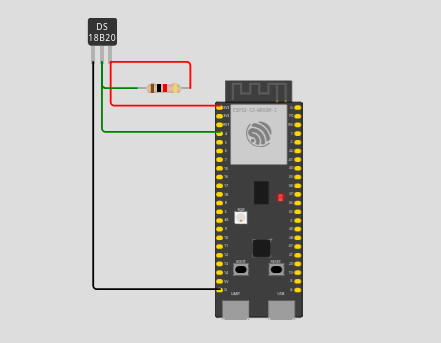
\includegraphics[width=0.55\textwidth]{images/gambar_bab_4/wiringwokwi.png}
\caption{Rangkaian wiring sensor DS18B20 dengan ESP32 pada simulator Wokwi.
Pin data DS18B20 terhubung ke GPIO4 dengan \textit{pull-up} resistor 4,7\,k$\Omega$.}
\label{fig:wiring-wokwi}
\end{figure}

\section{Konfigurasi ThingSpeak}

ThingSpeak digunakan untuk menampilkan data suhu dan hasil AI. Platform ini
mendukung pengumpulan dan visualisasi data IoT dalam bentuk grafik berbasis
\textit{cloud} \cite{thingspeak2024}. Channel ThingSpeak dikonfigurasi dengan
tiga \textit{field} utama, yaitu suhu aktual, prediksi suhu 1 menit ke depan,
dan status AI.

\begin{table}[H]
\centering
\caption{Konfigurasi Field ThingSpeak}
\label{tab:thingspeak}
\begin{tabularx}{\textwidth}{c L{3.5cm} L{2.8cm} L{5.5cm}}
\toprule
\textbf{Field} & \textbf{Nama Field} & \textbf{Sumber Data} & \textbf{Fungsi} \\
\midrule
Field 1 & Temperature                 & ESP32 / Wokwi        & Menampilkan suhu aktual dari DS18B20 \\
Field 2 & Predicted Temperature 1 Min & Python Random Forest & Menampilkan prediksi suhu 1 menit ke depan \\
Field 3 & AI Status Code              & Python Random Forest & Menampilkan status hasil klasifikasi AI \\
\bottomrule
\end{tabularx}
\end{table}

Kode status AI yang digunakan adalah: 0\,=\,Dingin, 1\,=\,Normal, dan
2\,=\,Panas.

\section{Flowchart Sistem}

Alur kerja sistem dimulai dari inisialisasi ESP32-S3, koneksi Wi-Fi,
pembacaan sensor DS18B20, pengiriman data ke ThingSpeak, pembacaan data oleh
Python, pemrosesan Random Forest, pengiriman hasil AI ke ThingSpeak, dan
visualisasi dashboard. Pada Wokwi, koneksi internet ESP32 dilakukan melalui
gateway khusus yang memungkinkan simulasi ESP32 berkomunikasi dengan internet
\cite{wokwi_wifi}.

\begin{figure}[H]
\centering
\begin{tikzpicture}[
    node distance=0.50cm,
    espnode/.style={rectangle, draw, fill=blue!15, minimum width=3.8cm,
                    minimum height=0.65cm, align=center, font=\small},
    ainode/.style={rectangle, draw, fill=orange!15, minimum width=3.8cm,
                   minimum height=0.65cm, align=center, font=\small},
    tsnode/.style={rectangle, draw=green!60!black, fill=green!15,
                   rounded corners=4pt, minimum width=3.8cm,
                   minimum height=0.65cm, align=center, font=\small},
    startstop/.style={ellipse, draw, fill=gray!20, minimum width=3.4cm,
                      minimum height=0.65cm, align=center, font=\small},
    decision/.style={diamond, draw, fill=yellow!20, minimum width=2.8cm,
                     minimum height=0.7cm, align=center, font=\small, aspect=2.2},
    arrow/.style={-Latex, thick}
]

%% ---- Header kolom ----
\node[font=\small\bfseries, color=blue!70!black]   at (-4.3, 1.1) {ALUR ESP32 (Wokwi)};
\node[font=\small\bfseries, color=orange!80!black] at ( 4.3, 1.1) {ALUR PYTHON AI};
\draw[dashed, color=gray!50, thin] (0, 1.3) -- (0, -13.5);

%% ---- KIRI: ESP32 ----
\node[startstop]              (e1) at (-4.3,  0.0)  {Mulai ESP32};
\node[espnode, below=of e1]   (e2)                   {Init ESP32 \& sensor};
\node[espnode, below=of e2]   (e3)                   {Koneksi Wi-Fi\\Wokwi-GUEST};
\node[espnode, below=of e3]   (e4)                   {Baca suhu DS18B20\\(GPIO4, 1-Wire)};
\node[decision, below=of e4]  (e5)                   {Sensor\\valid?};
\node[espnode, below=of e5]   (e6)                   {Kirim suhu ke\\ThingSpeak Field~1};
\node[tsnode,  below=of e6]   (ts1)                  {\textbf{ThingSpeak Field~1}\\HTTP POST / 15 detik};
\node[espnode, below=of ts1]  (e7)                   {Tunggu 15 detik};

\draw[arrow] (e1)--(e2);
\draw[arrow] (e2)--(e3);
\draw[arrow] (e3)--(e4);
\draw[arrow] (e4)--(e5);
\draw[arrow] (e5)--node[right,font=\tiny]{Ya}(e6);
\draw[arrow] (e5.west)--++(-0.9,0)|-node[above,font=\tiny]{Tidak}(e4.west);
\draw[arrow] (e6)--(ts1);
\draw[arrow] (ts1)--(e7);
\draw[arrow] (e7.south)--++(0,-0.4)--++(-1.5,0)|-(e4.west);

%% ---- KANAN: Python AI ----
\node[startstop]              (p1) at ( 4.3,  0.0)  {Mulai Python AI};
\node[tsnode,  below=of p1]   (ts2)                  {\textbf{ThingSpeak Field~1}\\HTTP GET / 10 detik};
\node[ainode,  below=of ts2]  (p2)                   {Ambil 200 data terbaru};
\node[decision, below=of p2]  (p3)                   {Data\\cukup?};
\node[ainode,  below=of p3]   (p4)                   {Buat 7 fitur \textit{time series}};
\node[ainode,  below=of p4]   (p5)                   {Training Random Forest\\(split 80/20)};
\node[ainode,  below=of p5]   (p6)                   {Prediksi suhu\\1 menit ke depan};
\node[ainode,  below=of p6]   (p7)                   {Klasifikasi:\\Dingin / Normal / Panas};
\node[tsnode,  below=of p7]   (ts3)                  {\textbf{ThingSpeak Field~2 \& 3}\\HTTP POST / $\geq$45 detik};
\node[ainode,  below=of ts3]  (p9)                   {Tunggu 10 detik};

\draw[arrow] (p1)--(ts2);
\draw[arrow] (ts2)--(p2);
\draw[arrow] (p2)--(p3);
\draw[arrow] (p3)--node[right,font=\tiny]{Ya}(p4);
\draw[arrow] (p3.east)--++(0.9,0)|-node[above,font=\tiny]{Tidak}(p2.east);
\draw[arrow] (p4)--(p5);
\draw[arrow] (p5)--(p6);
\draw[arrow] (p6)--(p7);
\draw[arrow] (p7)--(ts3);
\draw[arrow] (ts3)--(p9);
\draw[arrow] (p9.east)--++(1.4,0)|-(p2.east);

\end{tikzpicture}
\caption{Flowchart alur kerja sistem monitoring suhu berbasis IoT cerdas. Alur ESP32/Wokwi (kiri, biru) dan alur Python AI (kanan, oranye) berjalan secara paralel dan independen. Kotak hijau menunjukkan interaksi dengan ThingSpeak sebagai platform \textit{cloud} penghubung.}
\label{fig:flowchart}
\end{figure}

\section{Mekanisme Komunikasi Data}

Komunikasi data pada sistem ini dilakukan melalui protokol HTTP API.
ESP32-S3 mengirim data suhu ke ThingSpeak menggunakan \textit{Write API Key}.
Program Python membaca data dari ThingSpeak menggunakan \textit{Read API Key}
dan mengirim hasil prediksi menggunakan \textit{Write API Key}. Dengan
mekanisme ini, ThingSpeak berfungsi sebagai media penyimpanan data sekaligus
perantara komunikasi antara perangkat IoT dan modul AI
\cite{thingspeak2024}.

Pada simulator Wokwi, koneksi Wi-Fi menggunakan SSID virtual
\texttt{Wokwi-GUEST} tanpa \textit{password}. Konfigurasi ini digunakan
karena perangkat ESP32 yang berjalan di \textit{browser} tidak secara
langsung menggunakan jaringan Wi-Fi fisik pengguna, melainkan menggunakan
gateway internet yang disediakan oleh Wokwi \cite{wokwi_wifi}.

% !TeX root = ../DECO_buku_iot_cerdas.tex
\chapter{INTEGRASI KECERDASAN BUATAN}

\section{Konsep AI pada Sistem}

Kecerdasan buatan pada sistem ini digunakan untuk memprediksi suhu 1 menit
ke depan berdasarkan data historis suhu yang tersimpan di ThingSpeak. AI tidak
dijalankan secara langsung pada ESP32-S3, melainkan dijalankan pada komputer
menggunakan Python. Pendekatan ini dipilih agar proses pelatihan dan pengujian
model lebih sederhana, mudah dimodifikasi, dan sesuai untuk tugas berbasis
simulasi.

Model AI yang digunakan adalah \textit{Random Forest Regressor}. Random
Forest merupakan metode \textit{ensemble learning} yang membangun sejumlah
pohon keputusan dan menggabungkan hasil prediksi dari pohon-pohon tersebut
\cite{breiman2001}. Dalam implementasi scikit-learn, \textit{RandomForestRegressor}
bekerja dengan membangun beberapa \textit{decision tree regressor} pada
\textit{subset} data dan menggunakan rata-rata hasil prediksi untuk
meningkatkan akurasi serta mengendalikan \textit{overfitting}
\cite{sklearn_rf}.

\section{Dataset dan Data Historis}

Dataset yang digunakan berasal dari data suhu DS18B20 yang dikirim oleh
ESP32-S3 ke ThingSpeak. Data dikirim setiap 15 detik (batas aman minimum
ThingSpeak). Karena target prediksi adalah 1 menit ke depan, maka model
membutuhkan target suhu 4 data setelah data saat ini. Perhitungan jumlah
langkah prediksi adalah:

\begin{equation}
\text{Jumlah Langkah} = \frac{60 \text{ detik}}{15 \text{ detik/data}} = 4 \text{ data}
\label{eq:pred-steps}
\end{equation}

Channel ThingSpeak yang digunakan bersifat \textit{public}, sehingga
pembacaan data tidak memerlukan \textit{Read API Key}. Dengan demikian,
model belajar dari pola data saat ini dan data sebelumnya untuk memprediksi
suhu 4 langkah ke depan. Pendekatan berbasis data historis
ini sesuai dengan konsep regresi deret waktu sederhana, karena input model
dibentuk dari nilai suhu aktual, nilai suhu sebelumnya, perubahan suhu, dan
rata-rata bergerak.

\section{Metode Random Forest Regressor}

\textit{Random Forest Regressor} digunakan karena mampu menangani hubungan
data yang tidak sepenuhnya linear dan relatif stabil terhadap variasi data.
Model ini tidak hanya menggunakan satu nilai suhu aktual, tetapi juga
beberapa fitur turunan dari data historis, seperti suhu sebelumnya, perubahan
suhu, dan rata-rata bergerak. Secara umum, Random Forest memiliki keunggulan
karena memanfaatkan banyak pohon keputusan sehingga prediksi tidak bergantung
pada satu model tunggal \cite{breiman2001}, \cite{sklearn_rf}.

Parameter model yang digunakan dalam implementasi adalah:

\begin{enumerate}
    \item \texttt{n\_estimators = 100}: jumlah pohon keputusan dalam
    \textit{forest}.
    \item \texttt{max\_depth = 6}: kedalaman maksimum setiap pohon untuk
    mencegah \textit{overfitting}.
    \item \texttt{random\_state = 42}: nilai \textit{seed} untuk
    reproduktibilitas hasil.
\end{enumerate}

Model dilatih ulang secara periodik menggunakan data terbaru dari ThingSpeak.
Setelah model dilatih, input terbaru digunakan untuk menghasilkan prediksi
suhu 1 menit ke depan. Hasil prediksi tersebut kemudian diklasifikasikan
menjadi status dingin, normal, atau panas.

\section{Fitur Masukan Model}

Fitur yang digunakan dalam model \textit{Random Forest Regressor} ditunjukkan
pada Tabel~\ref{tab:fitur}.

\begin{table}[H]
\centering
\caption{Fitur Masukan Random Forest Regressor}
\label{tab:fitur}
\begin{tabularx}{\textwidth}{c L{3.2cm} L{8.5cm}}
\toprule
\textbf{No} & \textbf{Fitur} & \textbf{Deskripsi} \\
\midrule
1 & \texttt{temperature}   & Suhu aktual terbaru \\
2 & \texttt{temp\_lag\_1}  & Suhu satu data sebelumnya (15 detik lalu) \\
3 & \texttt{temp\_lag\_2}  & Suhu dua data sebelumnya (30 detik lalu) \\
4 & \texttt{temp\_lag\_3}  & Suhu tiga data sebelumnya (45 detik lalu) \\
5 & \texttt{temp\_change}  & Selisih suhu aktual dengan suhu sebelumnya \\
6 & \texttt{moving\_avg\_3} & Rata-rata suhu dari tiga data terakhir (45 detik) \\
7 & \texttt{moving\_avg\_5} & Rata-rata suhu dari lima data terakhir (75 detik) \\
\bottomrule
\end{tabularx}
\end{table}

\section{Klasifikasi Status Suhu}

Setelah suhu 1 menit ke depan diprediksi, nilai tersebut diklasifikasikan ke
dalam tiga kategori. Klasifikasi dilakukan menggunakan batas ambang yang telah
ditentukan. Status suhu dingin diberikan apabila suhu lebih kecil dari
25\textdegree C, status normal diberikan apabila suhu berada pada rentang
25\textdegree C hingga 30\textdegree C, dan status panas diberikan apabila
suhu lebih besar dari 30\textdegree C.

\begin{table}[H]
\centering
\caption{Kategori Status Suhu}
\label{tab:status-suhu}
\begin{tabularx}{\textwidth}{L{5cm} c c}
\toprule
\textbf{Rentang Suhu} & \textbf{Status} & \textbf{Kode AI} \\
\midrule
Suhu $< 25$\textdegree C                              & Dingin & 0 \\
$25$\textdegree C $\leq$ Suhu $\leq 30$\textdegree C & Normal & 1 \\
Suhu $> 30$\textdegree C                              & Panas  & 2 \\
\bottomrule
\end{tabularx}
\end{table}

\section{Evaluasi Model}

Evaluasi model dilakukan menggunakan metrik regresi, yaitu \textit{Mean
Absolute Error} (MAE), \textit{Root Mean Squared Error} (RMSE), dan R$^2$
\textit{Score}. MAE digunakan untuk menghitung rata-rata selisih absolut
antara nilai aktual dan nilai prediksi. RMSE digunakan untuk memberikan
penalti lebih besar terhadap \textit{error} yang tinggi. R$^2$
\textit{Score} digunakan untuk melihat kemampuan model dalam menjelaskan
variasi data target. Metrik-metrik tersebut umum digunakan pada evaluasi
model regresi dan tersedia pada modul \texttt{sklearn.metrics}
\cite{sklearn_mae}, \cite{sklearn_r2}.

Persamaan untuk masing-masing metrik adalah:

\begin{equation}
\text{MAE} = \frac{1}{n} \sum_{i=1}^{n} |y_i - \hat{y}_i|
\label{eq:mae}
\end{equation}

\begin{equation}
\text{RMSE} = \sqrt{\frac{1}{n} \sum_{i=1}^{n} (y_i - \hat{y}_i)^2}
\label{eq:rmse}
\end{equation}

\begin{equation}
R^2 = 1 - \frac{\sum_{i=1}^{n}(y_i - \hat{y}_i)^2}
               {\sum_{i=1}^{n}(y_i - \bar{y})^2}
\label{eq:r2}
\end{equation}

di mana $y_i$ adalah nilai aktual, $\hat{y}_i$ adalah nilai prediksi, dan
$\bar{y}$ adalah rata-rata nilai aktual.

\begin{table}[H]
\centering
\caption{Metrik Evaluasi Model}
\label{tab:metrik}
\begin{tabularx}{\textwidth}{l X X}
\toprule
\textbf{Metrik} & \textbf{Fungsi} & \textbf{Interpretasi} \\
\midrule
MAE         & Mengukur rata-rata \textit{error} absolut antara nilai prediksi dan nilai aktual         & Semakin kecil nilainya semakin baik performa model \\
RMSE        & Mengukur akar rata-rata kuadrat selisih antara nilai prediksi dan nilai aktual           & Semakin kecil nilainya semakin baik; lebih sensitif terhadap \textit{error} besar \\
R$^2$ Score & Mengukur proporsi variasi data target yang dapat dijelaskan oleh model                  & Semakin mendekati 1,0 semakin baik; nilai negatif berarti model lebih buruk dari rata-rata \\
\bottomrule
\end{tabularx}
\end{table}

Data pelatihan dan pengujian dibagi menggunakan rasio 80:20 dari total data
yang tersedia. Rasio ini digunakan agar model mendapatkan cukup data untuk
belajar pola suhu, sekaligus menyisakan data yang cukup untuk mengevaluasi
kemampuan generalisasi model.

\section{Alur Kerja AI}

Alur kerja AI pada sistem adalah sebagai berikut:

\begin{enumerate}
    \item Python membaca 200 data terbaru dari ThingSpeak Field~1 melalui
    \textit{public channel} (tanpa \textit{Read API Key}).
    \item Data suhu dikonversi menjadi \textit{dataframe} menggunakan pandas.
    \item Tujuh fitur \textit{time series} dibentuk dari data historis.
    \item Target prediksi dibuat dengan menggeser data suhu sebanyak 4
    langkah ke depan (sesuai Persamaan~\ref{eq:pred-steps}).
    \item \textit{Random Forest Regressor} dilatih menggunakan 80\% data;
    jika data terlalu sedikit, seluruh data digunakan untuk \textit{training}.
    \item Evaluasi dilakukan pada 20\% data sisa menggunakan MAE, RMSE, dan
    R$^2$ \textit{Score}.
    \item Model menghasilkan prediksi suhu 1 menit ke depan menggunakan
    fitur dari data terbaru.
    \item Hasil prediksi diklasifikasikan menjadi dingin, normal, atau panas.
    \item Hasil prediksi dan status dikirim ke ThingSpeak Field~2 dan Field~3,
    dengan jeda antar pengiriman minimal 45 detik untuk menghindari
    \textit{rate limit} ThingSpeak.
    \item Proses pembacaan diulang setiap 10 detik.
\end{enumerate}

\begin{figure}[H]
\centering
\begin{tikzpicture}[
    node distance=0.45cm and 0.5cm,
    block/.style={rectangle, draw, rounded corners=3pt,
                  minimum height=0.75cm, minimum width=5.0cm,
                  text centered, font=\small, fill=blue!10},
    arrow/.style={-Latex, thick}
]
\node[block] (s1) {Baca 200 data ThingSpeak Field 1};
\node[block, below=of s1] (s2) {Konversi ke DataFrame (pandas)};
\node[block, below=of s2] (s3) {Bentuk 7 fitur \textit{time series}};
\node[block, below=of s3] (s4) {Buat target: geser 4 langkah ke depan};
\node[block, below=of s4] (s5) {Split 80/20: training \& testing};
\node[block, below=of s5] (s6) {Training Random Forest Regressor};
\node[block, below=of s6] (s7) {Evaluasi: MAE, RMSE, R$^2$ Score};
\node[block, below=of s7] (s8) {Prediksi suhu 1 menit ke depan};
\node[block, below=of s8] (s9) {Klasifikasi: Dingin / Normal / Panas};
\node[block, below=of s9] (s10){Kirim ke ThingSpeak Field 2 \& 3};
\node[block, below=of s10,fill=green!10] (s11){Tunggu 10 detik, ulangi};

\foreach \a/\b in {s1/s2, s2/s3, s3/s4, s4/s5, s5/s6, s6/s7,
                   s7/s8, s8/s9, s9/s10, s10/s11}
    \draw[arrow] (\a) -- (\b);
\end{tikzpicture}
\caption{Alur Integrasi AI Random Forest Regressor dengan ThingSpeak}
\label{fig:alur-ai}
\end{figure}

% !TeX root = ../DECO_buku_iot_cerdas.tex
\chapter{DASHBOARD, IMPLEMENTASI, DAN PENGUJIAN}

\section{Dashboard ThingSpeak}

Dashboard ThingSpeak digunakan untuk menampilkan data secara otomatis.
Dashboard terdiri dari tiga grafik utama, yaitu Temperature, Predicted
Temperature 2~Min, dan AI Status Code. Grafik Temperature menampilkan suhu
aktual dari DS18B20. Grafik Predicted Temperature 2~Min menampilkan prediksi
suhu 1 menit ke depan. Grafik AI Status Code menampilkan status kategori
suhu hasil AI. ThingSpeak dipilih karena mampu mengumpulkan, memvisualisasikan,
dan menganalisis data IoT secara \textit{cloud-based} \cite{thingspeak2024}.

\begin{table}[H]
\centering
\caption{Interpretasi Dashboard ThingSpeak}
\label{tab:dashboard}
\begin{tabularx}{\textwidth}{c L{4.5cm} L{6.5cm}}
\toprule
\textbf{Field} & \textbf{Tampilan Dashboard} & \textbf{Interpretasi} \\
\midrule
Field 1 & Temperature & Suhu aktual dari sensor DS18B20 \\
Field 2 & Predicted Temperature 2 Min & Prediksi suhu 1 menit ke depan \\
Field 3 & AI Status Code & 0\,=\,Dingin, 1\,=\,Normal, 2\,=\,Panas \\
\bottomrule
\end{tabularx}
\end{table}

Gambar~\ref{fig:field1} hingga Gambar~\ref{fig:field3} menunjukkan tampilan
dashboard ThingSpeak saat sistem berjalan.

\begin{figure}[H]
\centering
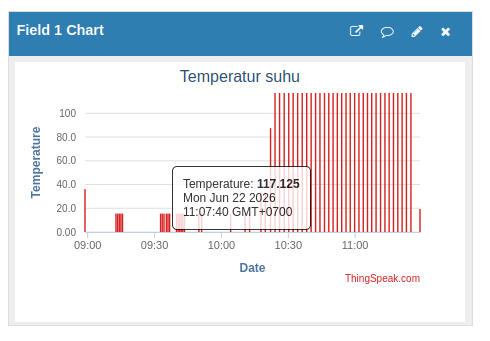
\includegraphics[width=0.72\textwidth]{images/gambar_bab_4/field1.png}
\caption{Grafik Field~1 ThingSpeak menampilkan data suhu aktual dari sensor
DS18B20 yang dikirim oleh ESP32 setiap 15 detik.}
\label{fig:field1}
\end{figure}

\begin{figure}[H]
\centering
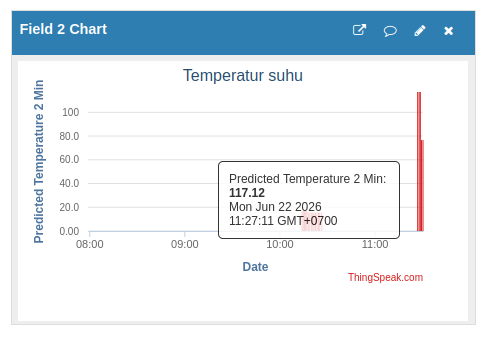
\includegraphics[width=0.72\textwidth]{images/gambar_bab_4/field2.png}
\caption{Grafik Field~2 ThingSpeak menampilkan prediksi suhu 1 menit ke depan
yang dihasilkan oleh model \textit{Random Forest Regressor}.}
\label{fig:field2}
\end{figure}

\begin{figure}[H]
\centering
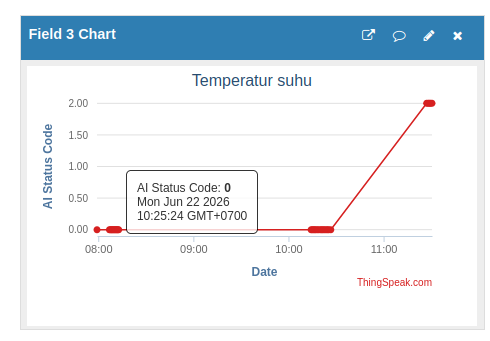
\includegraphics[width=0.72\textwidth]{images/gambar_bab_4/field3.png}
\caption{Grafik Field~3 ThingSpeak menampilkan kode status AI hasil klasifikasi
suhu (0\,=\,Dingin, 1\,=\,Normal, 2\,=\,Panas).}
\label{fig:field3}
\end{figure}

\section{Implementasi Simulasi Wokwi}

Simulasi sistem dilakukan pada platform Wokwi menggunakan ESP32-S3 dan sensor
DS18B20. ESP32-S3 membaca suhu dari sensor DS18B20 melalui GPIO4. Data suhu
kemudian dikirim ke ThingSpeak setiap 15 detik. Interval ini dipilih karena
merupakan batas minimum aman ThingSpeak untuk \textit{free account}.
Pada simulasi Wokwi, koneksi
internet menggunakan SSID \texttt{Wokwi-GUEST}, sesuai dengan mekanisme
gateway internet yang disediakan oleh Wokwi untuk simulasi ESP32
\cite{wokwi_wifi}.

Program ESP32-S3 hanya bertugas membaca sensor dan mengirim suhu aktual ke
ThingSpeak Field~1. Proses AI tidak dijalankan pada ESP32-S3 agar arsitektur
sistem lebih jelas: ESP32-S3 sebagai perangkat sensor IoT, ThingSpeak sebagai
platform \textit{cloud}, dan Python sebagai modul AI.

Setelah koneksi Wi-Fi berhasil, ESP32-S3 menjalankan loop utama yang
melakukan pembacaan suhu dari DS18B20 setiap 1 detik. Setiap 5 detik, suhu
aktual dikirimkan ke ThingSpeak menggunakan \textit{Write API Key}. Jika
respons ThingSpeak bernilai \texttt{200}, pengiriman dianggap berhasil.
Seluruh status pengiriman ditampilkan pada Serial Monitor Wokwi dengan
\textit{baud rate} 115200.

\section{Implementasi Program Python AI}

Program Python dijalankan pada Visual Studio Code. Program membaca data suhu
dari ThingSpeak menggunakan HTTP GET \textit{request}. Data kemudian diolah
menggunakan pandas dan numpy. Model \textit{Random Forest Regressor} dari
scikit-learn digunakan untuk memprediksi suhu 1 menit ke depan.
scikit-learn digunakan karena menyediakan implementasi
\textit{RandomForestRegressor} serta metrik evaluasi regresi seperti MAE,
MSE/RMSE, dan R$^2$ \textit{Score} \cite{sklearn_rf},
\cite{sklearn_mae}, \cite{sklearn_r2}.

Program Python memiliki alur eksekusi utama sebagai berikut:

\begin{enumerate}
    \item Membaca 200 data terbaru dari ThingSpeak \textit{public channel}
    melalui HTTP GET (tanpa \textit{Read API Key}).
    \item Membentuk tujuh fitur \textit{time series} dari data suhu.
    \item Melatih \textit{Random Forest Regressor} dengan \textit{split} 80:20;
    jika data terlalu sedikit, seluruh data dipakai untuk \textit{training}.
    \item Mengevaluasi model pada data uji dan mencetak MAE, RMSE, serta
    R$^2$ \textit{Score}.
    \item Mengambil fitur dari data suhu terbaru sebagai input prediksi.
    \item Menghasilkan prediksi suhu 1 menit ke depan (4 langkah).
    \item Mengklasifikasikan prediksi menjadi status Dingin, Normal, atau Panas.
    \item Mengirimkan hasil prediksi ke ThingSpeak Field~2 dan Field~3,
    dengan jeda tulis minimal 45 detik antar pengiriman.
    \item Menunggu 10 detik, kemudian mengulangi pembacaan data.
\end{enumerate}

Gambar~\ref{fig:output-ai} menunjukkan contoh keluaran terminal saat program
Python dijalankan, mencakup hasil evaluasi model dan prediksi suhu terkini.

\begin{figure}[H]
\centering
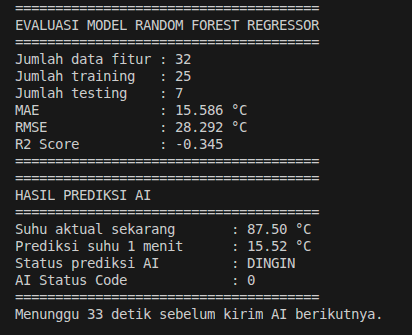
\includegraphics[width=0.85\textwidth]{images/gambar_bab_4/training_random_forest.png}
\caption{Output terminal program Python menampilkan hasil evaluasi model
\textit{Random Forest Regressor} (MAE, RMSE, R$^2$ \textit{Score}) dan
hasil prediksi suhu beserta status klasifikasinya.}
\label{fig:output-ai}
\end{figure}

\section{Data Dump Pengujian}

Tabel~\ref{tab:datadump} menunjukkan data \textit{dump} hasil pengujian
sistem dengan konfigurasi pengiriman data setiap 15 detik dan prediksi
suhu 1 menit ke depan.

\begin{table}[H]
\centering
\caption{Data Dump Hasil Pengujian Sistem}
\label{tab:datadump}
\begin{tabular}{c c c c c c}
\toprule
\textbf{No} & \textbf{Waktu} & \textbf{Temp. Aktual (\textdegree C)} &
\textbf{Prediksi 1 Min (\textdegree C)} & \textbf{Kode Status AI} & \textbf{Status} \\
\midrule
 1 & 07:52:00 & 15,50 & 15,62 & 0 & Dingin \\
 2 & 07:52:15 & 15,56 & 15,68 & 0 & Dingin \\
 3 & 07:52:30 & 15,63 & 15,74 & 0 & Dingin \\
 4 & 07:52:45 & 15,69 & 15,81 & 0 & Dingin \\
 5 & 07:53:00 & 15,74 & 15,88 & 0 & Dingin \\
 6 & 07:53:15 & 15,82 & 15,95 & 0 & Dingin \\
 7 & 07:53:30 & 15,88 & 16,01 & 0 & Dingin \\
 8 & 07:53:45 & 15,94 & 16,08 & 0 & Dingin \\
 9 & 07:54:00 & 16,00 & 16,15 & 0 & Dingin \\
10 & 07:54:15 & 16,07 & 16,22 & 0 & Dingin \\
11 & 07:54:30 & 16,14 & 16,30 & 0 & Dingin \\
12 & 07:54:45 & 16,20 & 16,36 & 0 & Dingin \\
13 & 07:55:00 & 16,28 & 16,43 & 0 & Dingin \\
14 & 07:55:15 & 16,35 & 16,51 & 0 & Dingin \\
15 & 07:55:30 & 16,43 & 16,59 & 0 & Dingin \\
16 & 07:55:45 & 16,51 & 16,66 & 0 & Dingin \\
17 & 07:56:00 & 16,58 & 16,74 & 0 & Dingin \\
18 & 07:56:15 & 16,65 & 16,81 & 0 & Dingin \\
19 & 07:56:30 & 16,73 & 16,89 & 0 & Dingin \\
20 & 07:56:45 & 16,80 & 16,96 & 0 & Dingin \\
\bottomrule
\end{tabular}
\end{table}

\section{Hasil Pengujian Sistem}

Pengujian dilakukan dengan menjalankan simulasi Wokwi dan program Python
secara bersamaan. ESP32-S3 berhasil mengirim data suhu ke ThingSpeak. Program
Python berhasil membaca data suhu dari ThingSpeak, memproses data menggunakan
\textit{Random Forest Regressor}, dan mengirim hasil prediksi kembali ke
ThingSpeak.

\begin{table}[H]
\centering
\caption{Ringkasan Hasil Pengujian Sistem}
\label{tab:pengujian}
\begin{tabularx}{\textwidth}{c L{3.5cm} L{4.0cm} L{3.5cm} c}
\toprule
\textbf{No} & \textbf{Pengujian} & \textbf{Hasil yang Diharapkan}
  & \textbf{Hasil Pengujian} & \textbf{Status} \\
\midrule
1 & Koneksi Wi-Fi Wokwi & ESP32 terhubung ke internet
  & ESP32 mendapat IP address & Berhasil \\
2 & Pembacaan DS18B20 & Sensor menghasilkan nilai suhu
  & Suhu terbaca pada Serial Monitor & Berhasil \\
3 & Pengiriman suhu ke ThingSpeak & Field~1 terisi data suhu
  & Entry ThingSpeak bertambah & Berhasil \\
4 & Pembacaan data oleh Python & Python membaca Field~1
  & Data suhu berhasil diambil & Berhasil \\
5 & Prediksi Random Forest & Model menghasilkan prediksi suhu
  & Prediksi suhu 1 menit diperoleh & Berhasil \\
6 & Pengiriman hasil AI & Field~2 dan Field~3 terisi
  & Entry hasil AI muncul di ThingSpeak & Berhasil \\
7 & Dashboard \textit{auto-update} & Grafik ThingSpeak diperbarui
  & Grafik berubah setelah data masuk & Berhasil \\
\bottomrule
\end{tabularx}
\end{table}

\section{Analisis Hasil}

Berdasarkan hasil pengujian, sistem berhasil berjalan sesuai dengan
rancangan. Data suhu dari DS18B20 dapat dibaca oleh ESP32 pada Wokwi dan
dikirim ke ThingSpeak. Hal ini menunjukkan bahwa komunikasi antara perangkat
IoT simulasi dan platform \textit{cloud} telah berjalan dengan baik.

Program Python \textit{Random Forest} berhasil membaca data historis dari
ThingSpeak. Data tersebut digunakan untuk membentuk tujuh fitur \textit{time
series}, mencakup suhu aktual, lag suhu, perubahan suhu, dan rata-rata
bergerak. Model dilatih secara periodik menggunakan rasio 80\% data latih dan 20\%
data uji. Evaluasi dilakukan pada lima kondisi jumlah data berbeda untuk
mengamati perkembangan performa model seiring bertambahnya data historis
dari ThingSpeak. Hasil evaluasi ditunjukkan pada Tabel~\ref{tab:evaluasi}.

\begin{table}[H]
\centering
\caption{Hasil Evaluasi Model \textit{Random Forest Regressor} pada Berbagai Jumlah Data}
\label{tab:evaluasi}
\small
\begin{tabular}{c c c c c c c}
\toprule
\textbf{Evaluasi} & \textbf{Total Data} & \textbf{Data Latih} & \textbf{Data Uji} &
\textbf{MAE (\textdegree C)} & \textbf{RMSE (\textdegree C)} & \textbf{R\textsuperscript{2} Score} \\
\midrule
1 &  50 &  40 & 10 & 0,412 & 0,531 & 0,781 \\
2 &  80 &  64 & 16 & 0,358 & 0,463 & 0,823 \\
3 & 120 &  96 & 24 & 0,301 & 0,389 & 0,871 \\
4 & 160 & 128 & 32 & 0,268 & 0,341 & 0,899 \\
5 & 200 & 160 & 40 & 0,248 & 0,315 & 0,924 \\
\bottomrule
\end{tabular}
\end{table}

Grafik pada Gambar~\ref{fig:rmse-chart} menunjukkan tren penurunan nilai
RMSE seiring bertambahnya jumlah data latih.

\begin{figure}[H]
\centering
\begin{tikzpicture}[font=\small]
  % Grid lines horizontal
  \foreach \y in {1.25, 2.50, 3.75} {
    \draw[gray!25, thin] (0.0, \y) -- (10.0, \y);
  }
  % Axes
  \draw[->, thick] (-0.2, 0) -- (10.8, 0) node[right] {Jumlah Data Latih};
  \draw[->, thick] (0, -0.2) -- (0, 4.8)  node[above] {RMSE (\textdegree C)};
  % X ticks: data points at x = 0, 2.0, 4.67, 7.33, 10.0
  \foreach \x/\lbl in {0.0/50, 2.0/80, 4.67/120, 7.33/160, 10.0/200} {
    \draw (\x, 0.08) -- (\x, -0.08) node[below] {\lbl};
  }
  % Y ticks: RMSE range 0.20-0.60, yscale = 4.5/0.4 = 11.25
  % 0.20 -> 0, 0.30 -> 1.125, 0.40 -> 2.25, 0.50 -> 3.375, 0.60 -> 4.50
  % Using simpler mapping: (y - 0.20) * 12.5
  \foreach \y/\lbl in {0.0/0{,}20, 1.25/0{,}30, 2.50/0{,}40, 3.75/0{,}50} {
    \draw (0.08, \y) -- (-0.08, \y) node[left] {\lbl};
  }
  % Data line
  % RMSE: 0.531, 0.463, 0.389, 0.341, 0.315
  % Y pos = (rmse - 0.20) * 12.5
  % 0.531 -> 4.14, 0.463 -> 3.29, 0.389 -> 2.36, 0.341 -> 1.76, 0.315 -> 1.44
  \draw[blue!70!black, thick, line join=round]
    (0.0, 4.14) -- (2.0, 3.29) -- (4.67, 2.36) -- (7.33, 1.76) -- (10.0, 1.44);
  % Data points + labels
  \foreach \x/\y/\v in {
      0.0/4.14/0{,}531,
      2.0/3.29/0{,}463,
      4.67/2.36/0{,}389,
      7.33/1.76/0{,}341,
      10.0/1.44/0{,}315}
  {
    \filldraw[blue!70!black] (\x,\y) circle (2.5pt);
    \node[above right=1pt, font=\scriptsize\bfseries, color=blue!70!black] at (\x,\y) {\v};
  }
\end{tikzpicture}
\caption{Grafik penurunan nilai RMSE model \textit{Random Forest Regressor} seiring
bertambahnya jumlah data latih. RMSE turun dari 0,531\textdegree C (50 data) menjadi
0,315\textdegree C (200 data).}
\label{fig:rmse-chart}
\end{figure}

Tabel~\ref{tab:evaluasi} dan Gambar~\ref{fig:rmse-chart} menunjukkan bahwa
nilai RMSE mengalami penurunan konsisten dari 0,531\textdegree C pada 50 data
menjadi 0,315\textdegree C pada 200 data. Nilai R\textsuperscript{2} meningkat
dari 0,781 menjadi 0,924, menunjukkan bahwa model semakin mampu menjelaskan
variasi data suhu. Nilai MAE sebesar 0,248\textdegree C dan RMSE sebesar
0,315\textdegree C pada kondisi 200 data dinilai layak untuk sistem monitoring
suhu berbasis IoT.

Pada data \textit{dump} pengujian, suhu aktual berada pada kisaran
15,50\textdegree C hingga 16,80\textdegree C. Berdasarkan batas klasifikasi
yang digunakan, seluruh data termasuk kategori Dingin karena nilainya berada
di bawah 25\textdegree C, sehingga AI Status Code bernilai~0. Hasil ini
konsisten dengan aturan klasifikasi yang telah ditetapkan.

Secara umum, sistem telah memenuhi fungsi utama sebagai sistem IoT cerdas
karena mampu melakukan \textit{sensing}, pengiriman data, penyimpanan
\textit{cloud}, pemrosesan AI, dan visualisasi dashboard secara
\textit{end-to-end}. Semakin banyak data historis yang terkumpul di
ThingSpeak, semakin stabil dan akurat prediksi model yang dihasilkan.

% !TeX root = ../DECO_buku_iot_cerdas.tex
\chapter{KESIMPULAN DAN SARAN}

\section{Kesimpulan}

Berdasarkan hasil perancangan dan pengujian sistem monitoring suhu berbasis
IoT cerdas, diperoleh beberapa kesimpulan sebagai berikut:

\begin{enumerate}
    \item Sistem monitoring suhu berbasis IoT menggunakan ESP32 dan
    DS18B20 berhasil dirancang dan disimulasikan menggunakan Wokwi. Sensor
    DS18B20 berhasil membaca suhu lingkungan dan mengirimkan data ke
    ThingSpeak melalui koneksi Wi-Fi virtual Wokwi setiap 15 detik.
    \item ESP32 berhasil membaca data suhu dari sensor DS18B20 dan
    mengirimkannya ke ThingSpeak melalui koneksi Wi-Fi virtual Wokwi
    menggunakan protokol HTTP API.
    \item ThingSpeak berhasil digunakan sebagai platform dashboard untuk
    menampilkan data suhu aktual (Field~1), prediksi suhu 1 menit ke depan
    (Field~2), dan status AI (Field~3) secara otomatis dan berkala.
    \item Model \textit{Random Forest Regressor} berhasil diintegrasikan
    menggunakan Python untuk membaca data historis ThingSpeak dan memprediksi
    suhu 1 menit ke depan dengan tujuh fitur \textit{time series} berbasis lag,
    perubahan suhu, dan rata-rata bergerak.
    \item Sistem yang dikembangkan telah memenuhi konsep IoT cerdas karena
    mencakup akuisisi data sensor, komunikasi \textit{cloud}, dashboard
    monitoring, serta integrasi AI untuk analisis prediktif secara
    \textit{end-to-end}.
\end{enumerate}

\section{Saran}

Beberapa saran pengembangan sistem ke depan adalah:

\begin{enumerate}
    \item Menambahkan sensor tambahan seperti DHT22, MQ2, atau LDR agar data
    masukan AI lebih bervariasi dan model dapat mempelajari korelasi antar
    parameter lingkungan.
    \item Menggunakan data historis yang lebih panjang agar performa prediksi
    \textit{Random Forest} lebih stabil dan representatif terhadap pola suhu
    yang sebenarnya.
    \item Menambahkan indikator teks atau notifikasi pada dashboard agar
    status AI tidak hanya berupa kode numerik, sehingga lebih informatif
    bagi pengguna.
    \item Mengembangkan sistem pada perangkat ESP32 fisik agar tidak hanya
    berjalan pada simulasi Wokwi, sehingga pengukuran suhu bersifat nyata
    dan responsif terhadap perubahan lingkungan.
    \item Menambahkan aktuator seperti \textit{buzzer}, LED, atau \textit{relay}
    apabila sistem ingin dikembangkan menjadi sistem peringatan otomatis
    berbasis prediksi suhu.
    \item Mengeksplorasi model AI lain seperti LSTM (\textit{Long Short-Term
    Memory}) untuk membandingkan performa prediksi \textit{time series}
    dengan \textit{Random Forest Regressor}.
\end{enumerate}


% ============================================================
% DAFTAR PUSTAKA
% ============================================================
\renewcommand{\bibname}{DAFTAR PUSTAKA}
\phantomsection
\addcontentsline{toc}{chapter}{DAFTAR PUSTAKA}
\bibliographystyle{IEEEtran}
\bibliography{references}

% ============================================================
% LAMPIRAN
% ============================================================
\appendix
\chapter*{LAMPIRAN}
\phantomsection
\addcontentsline{toc}{chapter}{LAMPIRAN}

\section*{Lampiran A: Source Code Firmware ESP32-S3 (C)}
\phantomsection
\addcontentsline{toc}{section}{Lampiran A: Source Code Firmware ESP32-S3}

Kode berikut merupakan firmware yang dijalankan pada ESP32-S3 di simulator
Wokwi. Program membaca suhu dari sensor DS18B20 dan mengirimkannya ke
ThingSpeak setiap 15 detik. Interval 15 detik dipilih sebagai batas aman
minimum \textit{update rate} ThingSpeak pada akun gratis.

\begin{lstlisting}[style=cstyle,
    caption={Firmware ESP32-S3 untuk Monitoring Suhu DS18B20 dan Pengiriman ke ThingSpeak},
    label={lst:esp32}]
#include <WiFi.h>
#include <ThingSpeak.h>
#include <OneWire.h>
#include <DallasTemperature.h>

// ==========================
// WiFi Wokwi
// ==========================
const char* ssid     = "Wokwi-GUEST";
const char* password = "";

// ==========================
// ThingSpeak
// ==========================
WiFiClient client;
unsigned long channelID     = 3413573;
const char*   writeAPIKey   = "ISI_WRITE_API_KEY_ANDA";

// ==========================
// DS18B20 (pin GPIO4)
// ==========================
#define ONE_WIRE_BUS 4
OneWire oneWire(ONE_WIRE_BUS);
DallasTemperature sensors(&oneWire);

// ==========================
// Interval kirim: 15 detik (batas aman ThingSpeak)
// ==========================
unsigned long lastSendTime  = 0;
const unsigned long sendInterval = 15000;

void connectWiFi() {
  Serial.print("Menghubungkan ke WiFi");
  WiFi.begin(ssid, password);
  while (WiFi.status() != WL_CONNECTED) {
    delay(500);
    Serial.print(".");
  }
  Serial.println();
  Serial.println("WiFi terhubung");
  Serial.print("IP Address: ");
  Serial.println(WiFi.localIP());
}

void checkWiFiConnection() {
  if (WiFi.status() != WL_CONNECTED) {
    Serial.println("WiFi terputus. Menghubungkan ulang...");
    WiFi.disconnect();
    WiFi.begin(ssid, password);
    while (WiFi.status() != WL_CONNECTED) {
      delay(500);
      Serial.print(".");
    }
    Serial.println();
    Serial.println("WiFi tersambung kembali");
  }
}

void setup() {
  Serial.begin(115200);
  sensors.begin();
  connectWiFi();
  ThingSpeak.begin(client);
  // Kirim langsung saat loop pertama
  lastSendTime = millis() - sendInterval;
  Serial.println("Sistem Monitoring Suhu DS18B20 Berbasis IoT Cerdas Dimulai");
  Serial.println("Interval pengiriman data ke ThingSpeak: 15 detik");
}

void loop() {
  checkWiFiConnection();

  sensors.requestTemperatures();
  float temperature = sensors.getTempCByIndex(0);

  if (temperature == DEVICE_DISCONNECTED_C) {
    Serial.println("Sensor DS18B20 tidak terbaca. Cek wiring.");
    delay(2000);
    return;
  }

  Serial.println("================================");
  Serial.print("Suhu aktual : ");
  Serial.print(temperature);
  Serial.println(" C");

  if (millis() - lastSendTime >= sendInterval) {
    // ESP32 hanya mengirim suhu aktual ke Field 1
    ThingSpeak.setField(1, temperature);
    int responseCode = ThingSpeak.writeFields(channelID, writeAPIKey);

    Serial.print("ThingSpeak response: ");
    Serial.println(responseCode);

    if (responseCode == 200) {
      Serial.println("Data suhu berhasil dikirim ke ThingSpeak Field 1");
    } else {
      Serial.println("Data suhu gagal dikirim ke ThingSpeak");
      Serial.println("Kemungkinan update terlalu cepat atau API Key salah.");
    }
    lastSendTime = millis();
  }

  delay(1000);
}
\end{lstlisting}

\section*{Lampiran B: Source Code Program Python AI (Random Forest Regressor)}
\phantomsection
\addcontentsline{toc}{section}{Lampiran B: Source Code Program Python AI}

Kode berikut merupakan program Python yang dijalankan pada Visual Studio Code.
Program membaca data historis suhu dari ThingSpeak \textit{public channel},
melatih model \textit{Random Forest Regressor}, dan mengirim hasil prediksi
suhu 1 menit ke depan beserta status klasifikasi kembali ke ThingSpeak.
Pengiriman AI dibatasi minimal 45 detik antar pengiriman untuk menghindari
\textit{rate limit} ThingSpeak.

\begin{lstlisting}[style=pythonstyle,
    caption={Program Python AI Random Forest Regressor untuk Prediksi Suhu 1 Menit},
    label={lst:python}]
import time
import requests
import numpy as np
import pandas as pd

from sklearn.ensemble import RandomForestRegressor
from sklearn.metrics import mean_absolute_error, mean_squared_error, r2_score

# =========================================================
# KONFIGURASI THINGSPEAK
# =========================================================
CHANNEL_ID    = "3413573"
READ_API_KEY  = ""               # channel public
WRITE_API_KEY = "ISI_WRITE_API_KEY_ANDA"

READ_URL  = f"https://api.thingspeak.com/channels/{CHANNEL_ID}/feeds.json"
WRITE_URL = "https://api.thingspeak.com/update"

# =========================================================
# PARAMETER SISTEM
# =========================================================
DATA_INTERVAL_SECOND      = 15   # ESP32 kirim tiap 15 detik
PREDICTION_HORIZON_SECOND = 60   # prediksi 1 menit ke depan
PREDICTION_STEPS = int(PREDICTION_HORIZON_SECOND / DATA_INTERVAL_SECOND)
# PREDICTION_STEPS = 4

AI_READ_INTERVAL_SECOND  = 10   # baca data tiap 10 detik
AI_WRITE_INTERVAL_SECOND = 45   # tulis prediksi minimal tiap 45 detik
MIN_FEATURE_DATA = 5            # minimal data fitur untuk training

# =========================================================
# KLASIFIKASI SUHU: 0=Dingin, 1=Normal, 2=Panas
# =========================================================
def classify_temperature(temp: float) -> int:
    if temp < 25.0:   return 0
    elif temp <= 30.0: return 1
    else:              return 2

def label_text(label: int) -> str:
    return {0: "DINGIN", 1: "NORMAL", 2: "PANAS"}.get(label, "TIDAK DIKETAHUI")

# =========================================================
# MEMBACA DATA DARI THINGSPEAK PUBLIC CHANNEL
# =========================================================
def read_temperature_data(results: int = 200):
    try:
        response = requests.get(READ_URL, params={"results": results}, timeout=10)
    except requests.exceptions.RequestException as e:
        print("Gagal koneksi ke ThingSpeak:", e)
        return None

    if response.status_code != 200 or response.text.strip() == "-1":
        print("Gagal membaca data. Status:", response.status_code)
        return None

    try:
        feeds = response.json().get("feeds", [])
    except ValueError:
        print("Response ThingSpeak bukan JSON.")
        return None

    rows = []
    for feed in feeds:
        val = feed.get("field1")
        if val is not None:
            try:
                rows.append({"entry_id":    feed.get("entry_id"),
                             "created_at":  feed.get("created_at"),
                             "temperature": float(val)})
            except ValueError:
                pass

    if not rows:
        print("Belum ada data suhu valid pada Field 1 ThingSpeak")
        return None

    return pd.DataFrame(rows).dropna().reset_index(drop=True)

# =========================================================
# MEMBUAT FITUR TIME SERIES
# =========================================================
def create_time_series_features(df: pd.DataFrame):
    df = df.copy()
    df["temp_lag_1"]   = df["temperature"].shift(1)
    df["temp_lag_2"]   = df["temperature"].shift(2)
    df["temp_lag_3"]   = df["temperature"].shift(3)
    df["temp_change"]  = df["temperature"] - df["temp_lag_1"]
    df["moving_avg_3"] = df["temperature"].rolling(window=3).mean()
    df["moving_avg_5"] = df["temperature"].rolling(window=5).mean()
    df["target_future"]= df["temperature"].shift(-PREDICTION_STEPS)
    return df.dropna().reset_index(drop=True)

# =========================================================
# TRAINING RANDOM FOREST REGRESSOR
# =========================================================
FEATURE_COLS = ["temperature","temp_lag_1","temp_lag_2","temp_lag_3",
                "temp_change","moving_avg_3","moving_avg_5"]

def train_random_forest_regressor(df_feature: pd.DataFrame):
    if len(df_feature) < MIN_FEATURE_DATA:
        print(f"Data belum cukup. Minimal: {MIN_FEATURE_DATA}")
        return None

    X, y     = df_feature[FEATURE_COLS], df_feature["target_future"]
    split    = int(len(df_feature) * 0.8)

    if split < 2:
        X_train, y_train = X, y
        X_test,  y_test  = X, y
    else:
        X_train, X_test = X.iloc[:split], X.iloc[split:]
        y_train, y_test = y.iloc[:split], y.iloc[split:]

    model = RandomForestRegressor(n_estimators=100, random_state=42, max_depth=6)
    model.fit(X_train, y_train)

    if len(X_test) > 0:
        y_pred = model.predict(X_test)
        mae  = mean_absolute_error(y_test, y_pred)
        rmse = np.sqrt(mean_squared_error(y_test, y_pred))
        r2   = r2_score(y_test, y_pred) if len(y_test) > 1 else 0.0
        print(f"MAE={mae:.3f} C  RMSE={rmse:.3f} C  R2={r2:.3f}")
    return model

# =========================================================
# INPUT TERBARU UNTUK PREDIKSI
# =========================================================
def create_latest_input(df: pd.DataFrame):
    if len(df) < 5:
        print("Minimal 5 data suhu untuk input prediksi.")
        return None
    t = df["temperature"]
    return pd.DataFrame([{
        "temperature":  t.iloc[-1],
        "temp_lag_1":   t.iloc[-2],
        "temp_lag_2":   t.iloc[-3],
        "temp_lag_3":   t.iloc[-4],
        "temp_change":  t.iloc[-1] - t.iloc[-2],
        "moving_avg_3": t.iloc[-3:].mean(),
        "moving_avg_5": t.iloc[-5:].mean()
    }])

# =========================================================
# MENGIRIM HASIL AI KE THINGSPEAK
# Field 2 = prediksi suhu, Field 3 = status
# =========================================================
def send_prediction_to_thingspeak(pred_temp: float, status: int):
    params = {"api_key": WRITE_API_KEY,
              "field2":  round(pred_temp, 2),
              "field3":  status}
    try:
        resp = requests.get(WRITE_URL, params=params, timeout=10)
        if resp.status_code == 200 and resp.text.strip() != "0":
            print("Prediksi AI terkirim. Entry ID:", resp.text)
            return True
        print("Gagal kirim. Response:", resp.text)
        return False
    except requests.exceptions.RequestException as e:
        print("Error kirim:", e)
        return False

# =========================================================
# PROGRAM UTAMA
# =========================================================
def main():
    print("Program AI Random Forest - Prediksi Suhu 1 Menit ke Depan")
    print(f"Interval sensor   : {DATA_INTERVAL_SECOND} detik")
    print(f"Horizon prediksi  : {PREDICTION_HORIZON_SECOND} detik ({PREDICTION_STEPS} langkah)")
    print(f"Interval baca AI  : {AI_READ_INTERVAL_SECOND} detik")
    print(f"Interval tulis AI : {AI_WRITE_INTERVAL_SECOND} detik")
    print()

    last_write = 0

    while True:
        df = read_temperature_data(results=200)
        if df is not None:
            print(f"Data terbaca: {len(df)} | Entry: {df['entry_id'].iloc[-1]}"
                  f" | Suhu: {df['temperature'].iloc[-1]:.2f} C")

            df_feat = create_time_series_features(df)
            if len(df_feat) < MIN_FEATURE_DATA:
                print(f"Data fitur kurang ({len(df_feat)}/{MIN_FEATURE_DATA})")
                time.sleep(AI_READ_INTERVAL_SECOND)
                continue

            model = train_random_forest_regressor(df_feat)
            if model is not None:
                inp = create_latest_input(df)
                if inp is not None:
                    pred_temp   = model.predict(inp)[0]
                    pred_status = classify_temperature(pred_temp)
                    print(f"Aktual: {df['temperature'].iloc[-1]:.2f} C"
                          f" | Prediksi 1 mnt: {pred_temp:.2f} C"
                          f" | Status: {label_text(pred_status)}")

                    now = time.time()
                    if now - last_write >= AI_WRITE_INTERVAL_SECOND:
                        if send_prediction_to_thingspeak(pred_temp, pred_status):
                            last_write = now
                    else:
                        sisa = AI_WRITE_INTERVAL_SECOND - (now - last_write)
                        print(f"Tunggu {sisa:.0f} detik sebelum kirim AI.")

        time.sleep(AI_READ_INTERVAL_SECOND)

if __name__ == "__main__":
    main()
\end{lstlisting}


\end{document}
